\rhead{\itshape Approches de l’IoT dans la maison intelligente}

\chapter{Approches de l’IoT dans la maison intelligente}
\section{Introduction}
Dans ce chapitre, nous allons donner un aperçu sur l’évolution des constructions des maisons jusqu’à la naissance du terme maison intelligente (Smart home), ensuite nous allons définier  ce qui est une maison intelligente, En plus, nous allons présenter un état de l’art sur les approches utilisant la technologie de l’Internet des objets dans un smart house.
\section{Historique}
Les constructions ont évolué en fonction des besoins de l’homme, l'homme de l'histoire et nomade et se déplace au gré des saisons et des migrations animales, pour se mettre l'abri il fabrique des huttes faites de branchages d'ossements et de peau. 
\begin{figure}[H]
    \centering
    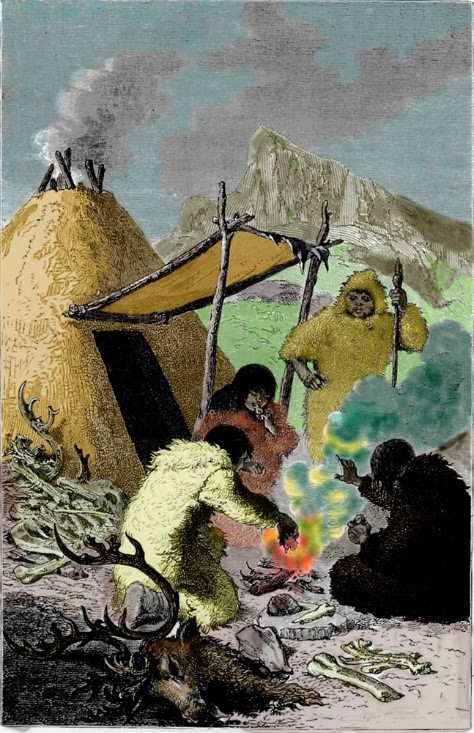
\includegraphics[scale=1]{chap1/chap31.jpg}
    \caption{Maisons de Néandertal}
    \label{chap31}
\end{figure}


Il y a environ 12 mille ans les hommes inventent l'élevage et l'agriculture, n'ayant plus besoin de se déplacer pour trouver leur nourriture, ils bâtissent des habitats fixes et se regroupent dans les premiers villages dont les maisons sont rondes construite en bois ou en terre et recouvertes de feuillages,
\begin{figure}[H]
    \centering
    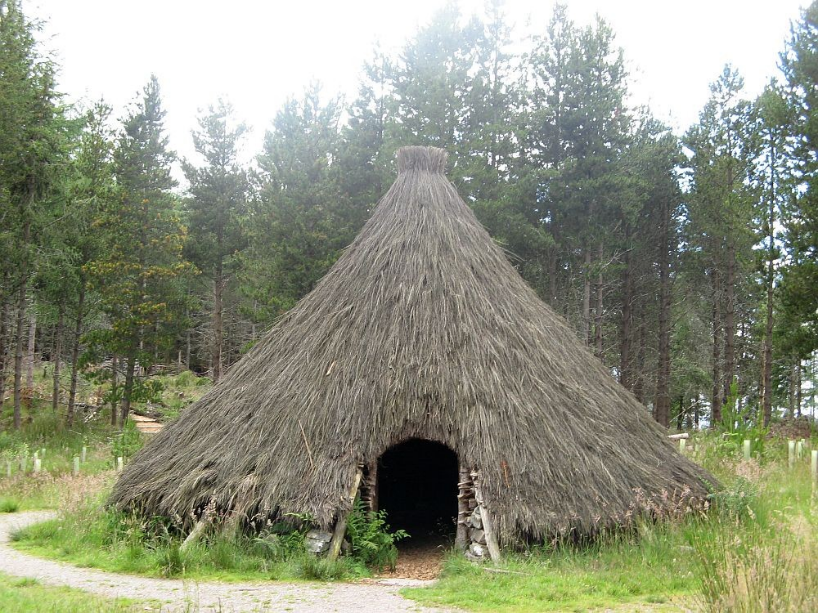
\includegraphics[scale=1]{chap1/chap32.png}
   \caption{Maisons rondes de bois}
    \label{chap32}
\end{figure}

C’est en Mésopotamie il y a cinq mille ans que naissent les premières villes progressivement les maisons deviennent rectangulaire ou carrés formé ou pratiques pour être cloisonné en différents espaces et permettent d'assembler les maisons les unes contre les autres autour de petites rues. 
\begin{figure}[H]
    \centering
    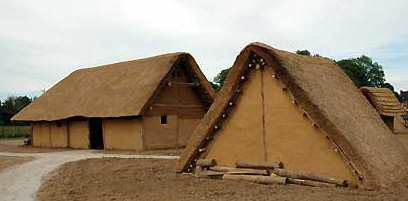
\includegraphics[scale=1]{chap1/chap33.png}
   \caption{Maisons rectangulaires ou carrées}
    \label{chap33}
\end{figure}


En Egypte les maisons traditionnelles sont construites en briques de terre et en paille et possèdent déjà  plusieurs pièces plus tard les riches se font construire des demeures de plusieurs étages, peu les grandes villes du bassin méditerranéen s'organisant en quartier, séparant  habitations ateliers culte religieux marché; elles sont déjà pourvus de canalisations qui assurent l'arrivée d'eau dans les maisons.

\begin{figure}[H]
    \centering
    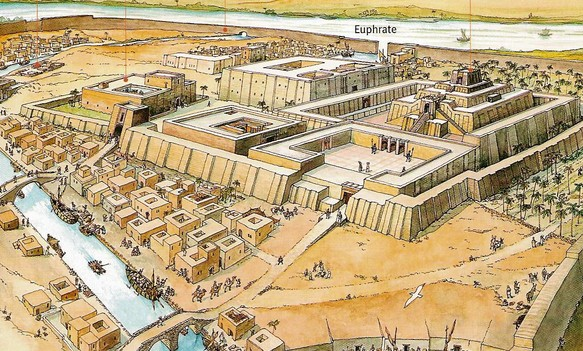
\includegraphics[scale=0.8]{chap1/chap34.png}
   \caption{Une grande ville  méditerranéen}
    \label{chap34}
\end{figure}

La maison gauloise est construite avec les matériaux disponibles proximité du bois pour sa structure, il faut de la charpente du torchis qui est une mélange de terre et de paille pour les murs, de la paille pour le toit, sans fenêtre cette maison est sombre, et est constitué d'une pièce qui accueille un foyer pour s'éclairer et cuisine et d'une réserve  provisions et d'un grenier plus chaud pour y dormir.


\begin{figure}[H]
    \centering
    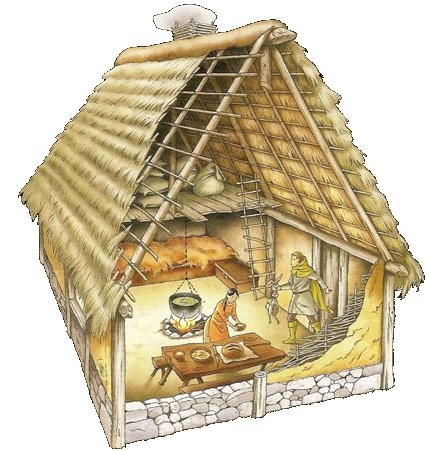
\includegraphics[scale=0.7]{chap1/chap35.png}
   \caption{Modèle d'une maison gauloise}
    \label{chap35}
\end{figure}


En Europe c'est  à partir du $12^{éme}$ siècle que la pierre remplace peu  à  peu le bois jugé trop fragile face aux incendies dans les bourgs et les villes. L'époque est propice pour la construction de fortifications devant assurer la défense de la population en cas d'attaque, la cité médiévale compte de nombreux édifices, habitations, ateliers, boutiques, tandis que les plus riches habitent des logements spacieux et confortables les pauvres vivent dans des pièces étroites sombre et souvent insalubres.


\begin{figure}[H]
    \centering
    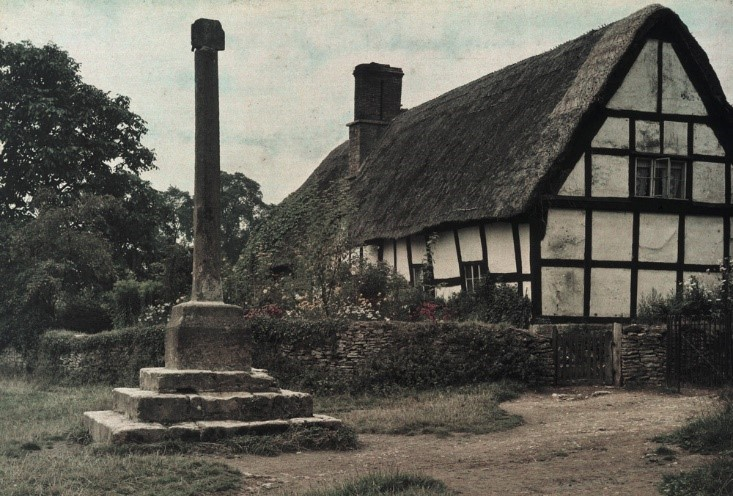
\includegraphics[scale=1.2]{chap1/chap36.jpg}
   \caption{Maison de la 12éme siècle}
    \label{chap36}
\end{figure}

Au $16^{éme}$ siècle, l’architecture renaissance venus d’Italie se propage en Europe, les riches demeures rappelle l'architecture romaine par leurs formes leurs colonnes leur proportion les façades sont plus régulières et pourvue de grandes fenêtres en verre. Au $19^{éme}$ siècle les grands industriels implantent des cités ouvrières pour loger leur main d'œuvre proximité des usines, ces petites maisons en briques sont toutes identiques et sans confort.

\begin{figure}[H]
    \centering
    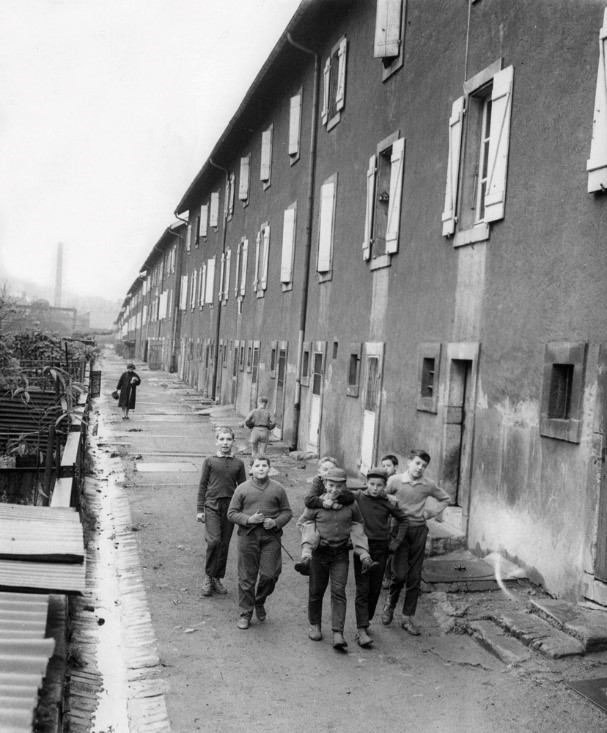
\includegraphics[scale=1]{chap1/chap37.jpg}
   \caption{Cité ouvrière}
    \label{chap36}
\end{figure}

Le $20^{éme}$ siècle est marqué par l'exode rural et le développement des villes. Pour faire face au manque de place on construit en hauteur c'est l'ère des gratte-ciel avec des matériaux nouveau, béton,  acier, aluminium, verre. Dans les banlieues apparaissent des tours et des barres d'immeubles, les habitants de plus en plus éloignés des centres villes et passent beaucoup de temps dans les transports.

\begin{figure}[H]
    \centering
    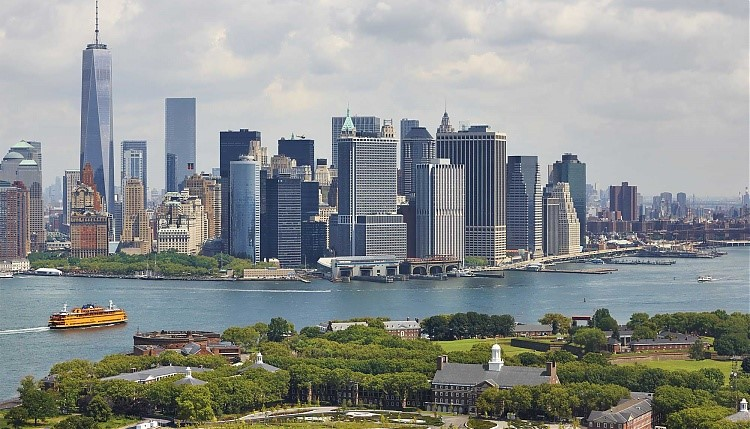
\includegraphics[scale=0.5]{chap1/chap38.jpg}
   \caption{Cité du $20^{éme}$ siècle}
    \label{chap36}
\end{figure}


Aujourd’hui on cherche à  diminuer notre consommation d'énergie ce qui nécessite de réduire les déplacements en voiture et de construire des logements écologiques, pratiques, plus économes, confortable et respectueux de l'environnement.


Cette évolution des constructions a été toujours liée avec le déroulement des besoins humains, et avec l'émergence de l’IT comme concept de confort, il est devenu nécessaire de le joindre dans la vie quotidienne pour fournir un environnement plus confortable pour l'habitant, Ces dernières années, un nouveau type des maisons a vu le jour, que nous appelons les maisons automatique et les maisons intelligentes (smart home) .


Le terme «maisons intelligentes » a été utilisé pour la première fois de manière officielle en 1984 par l'Association américaine des constructeurs de maisons, bien que les premières "maisons câblées" aient été en fait construites par des amateurs au début des années 1960. Et ce développement est la clé de ce que l'on entend par "maisons intelligentes". Car une maison n'est pas intelligente parce qu'elle est bien construite, ni parce qu'elle utilise efficacement l'espace ; ni parce qu'elle est écologique, en utilisant l'énergie solaire et en recyclant les eaux usées, par exemple. Une maison intelligente peut inclure ces objets, et c'est d'ailleurs souvent le cas, mais ce qui la rend intelligente, ce sont les technologies interactives qu'elle contient.


Les objets d'une maison intelligente sont reliés entre eux et accessibles par un point d’accès (Gateway) - un smartphone, une tablette, un ordinateur portable ou une console de jeu. Les serrures de porte, les télévisions, les thermostats, les moniteurs domestiques, les caméras, les lumières et même les appareils tels que le réfrigérateur peuvent être contrôlés par un seul système domotique. Le système est installé sur un téléphone portable ou un autre appareil en réseau, et l'utilisateur peut créer des horaires pour que certains changements prennent effet.


En 2016, le marché mondial de la domotique était estimé à environ 36 milliards de dollars, et avec l'adoption croissante des appareils fonctionnant sur Internet, on prévoit que le marché pourrait atteindre des revenus de l'ordre de 80 milliards de dollars d'ici 2020. La croissance du marché de la domotique au sens large a toutefois été confrontée à des défis en raison de sa nature axée sur la commodité, plutôt que sur la nécessité.
\section{Définition de la maison intelligente}
Une maison intelligente est une résidence équipée d'un réseau de communication, reliant des capteurs, des appareils ménagers et d'autres dispositifs électroniques et électriques, qui peut être surveillée, accédée ou contrôlée à distance et qui fournissent des services qui répondent aux besoins de ses habitants\cite{chap31}.


Une "maison intelligente" peut être définie comme une résidence équipée de technologies informatiques qui anticipent et répondent aux besoins des occupants, en s'efforçant de promouvoir leur confort, leur commodité, leur sécurité et leurs loisirs grâce à la gestion de la technologie à l'intérieur de la maison et aux connexions avec le monde extérieur \cite{chap32}.


Une maison intelligente est une installation domestique pratique où les objets et les dispositifs peuvent être automatiquement contrôlés à distance depuis n'importe quel endroit connecté à Internet dans le monde à l'aide d'un smartphone ou d'un autre dispositif en réseau. Les objets d'une maison intelligente sont interconnectés par internet et l'utilisateur peut contrôler des fonctions telles que l'accès sécurisé à la maison, la température, l'éclairage et le cinéma maison. Les termes connexes comprennent la "domotique" et le "bâtiment intelligent". 

\section{Travaux connexes}

Afin de mieux analyser des travaux connexes, nous avons detaillé points suivants :
Travaux exploitant l’IoT dans le smart house sans  le cloud,Travaux exploitant l’IoT dans le smart house via le cloud, Travaux sur les architecture des smart houses, Travaux sur les architecture des objets et Travaux sur les robots basés internet des objets.

\subsection{Travaux exploitant l’IoT dans le smart house sans le cloud}
Dans \cite{chap37}, les auteurs ont proposé un système de contrôle intelligent basé sur les technologies de l'internet des objets. Le système de contrôle domestique intelligent utilise un contrôleur central intelligent pour configurer un réseau de capteurs et d'actionneurs sans fil à fréquence radio 433 MHz (WSAN). Une série de modules de contrôle, tels que des modules de commutation, des modules de contrôle de radiofréquence, ont été développés dans le WSAN pour contrôler directement tous les types d'appareils ménagers. Les serveurs d'applications, les ordinateurs clients, les tablettes ou les smartphones peuvent communiquer avec le contrôleur central intelligent via un routeur sans fil via une interface Wi-Fi. Puisqu'il a WSAN comme couche de contrôle inférieure, un appareil peut être ajouté ou retiré du système de contrôle très facilement. Le système de contrôle intelligent englobe les fonctions de surveillance, de contrôle et de gestion des appareils, de sécurité à domicile, de statistiques et d'analyses énergétiques.

Dans \cite{chap38}, les auteurs ont proposé un système domotique télécommandé à faible coût et convivial présenté à l'aide de la carte Arduino, du module Bluetooth, du smartphone, du capteur à ultrasons et du capteur d'humidité. Une application pour smartphone est utilisée dans le système proposé qui permet aux utilisateurs de contrôler jusqu'à 18 appareils, y compris des appareils électroménagers et des capteurs à l'aide de la technologie Bluetooth, le système proposé est un système domotique à usage général. Qui peut facilement être mis en œuvre dans une maison existante, le système suggéré à plus de fonctionnalités que les systèmes domotiques conventionnels tels qu'un capteur à ultrasons est utilisé pour la détection du niveau d'eau et un capteur d'humidité du sol sont utilisés pour un système d'irrigation automatique des plantes. Les auteurs décrivent également l'architecture matérielle et logicielle d'un système, ses travaux futurs et sa portée.


\subsection{Travaux exploitant l’IoT dans le smart house via le cloud }
Dans \cite{chap33}, les auteurs ont proposé un prototype d’une maison intelligente basée sur des systèmes embarqués et internet des objets et des technologies de cloud computing afin de proposer une vie plus intelligente et plus confortable pour les utilisateurs finaux, pour la communication locale entre la passerelle et les différents nœuds dont ils ont utilisé les technologies de communications économiques low-cost et low-power, ZigBee basé sur la norme 802.15.4 et les technologies Bluetooth sont basées sur la norme IEEE 802.15.1, ce prototype implémenté par une carte Raspberry Pi connectée au coordinateur XBee utilisé comme passerelle IoT basée sur Zigbee et deux nœuds. La chambre et la cuisine qui contiennent chacune un Arduino connecté au module routeur XBee. Chaque nœud intelligent dispose d'un ensemble des équipements et des capteurs. La maison intelligente contrôlée par une application de bureau Web basée sur le langage PHP. La plate-forme Cloud utilisée pour enregistrer les actions quotidiennes effectuées par l'utilisateur.


Dans \cite{chap34}, les auteurs ont proposé une approche d'une maison intelligente en intégrant l'Internet des objets (IoT) aux services Web et au cloud computing, cette approche se concentre sur l'intégration de l'intelligence dans les capteurs et les actionneurs utilisant la plate-forme Arduino; mettre en réseau des objets intelligents en utilisant la technologie Zigbee; faciliter les interactions avec les objets intelligentes en utilisant les services Cloud; améliorer l'efficacité de l'échange de données en utilisant le format de données JSON. Cette approche a été mise en œuvre en utilisant la carte Arduino comme carte microcontrôleur pour programmer divers types de capteurs / actionneurs et technologies de communication tels que RFID et ZigBee et basée sur le cloud computing qui fournit des ressources de stockage et de calcul pour implémenter des applications Web.


Dans \cite{chap35},les auteurs ont proposé la structure de la maison intelligente basée sur le Cloud Computing, qui aide à réduire la charge de travail locale et les utilisateurs obtiennent directement les informations en temps réel via un navigateur Web. De plus, ils construisent la plateforme expérimentale pour valider la structure de la maison intelligente basée sur le Cloud Computing, les résultats expérimentaux montrent que la structure proposée d'une maison intelligente est plus pratique, flexible, à haut rendement et à faible coût. L'architecture proposée implémentée par Raspberry PI et un service Web domestique intelligent basé sur le Cloud Computing pour les utilisateurs sur la plate-forme PaaS fournie par Google.les données distribuées sont stockées grâce au service d'interface JDO basé sur Google App Engine, et le convertisseur de protocole réalise la transition entre le ZigBee, le Bluetooth et le port série.


Dans \cite{chap36} , les auteurs ont proposé une surveillance et une automatisation de maisons solaires basées sur la plate-forme EmonCMS qui utilise un serveur cloud pour collecter des données à partir de nœuds de capteurs en utilisant le principe IoT. Les données collectées peuvent être affichées, archivées ou traitées et utilisées pour contrôler les appareils dans la maison. Le NodeMCU combiné à l'ESP2866 a été utilisé comme unité de traitement principale qui collecte les données des capteurs, les traiter puis les télécharger sur le serveur cloud EmonCMS. Le NodeMCU peut également lire les données et les commandes du même serveur et contrôler les dispositifs de commutation. Il s'agit d'un système complet de surveillance et d'automatisation de la maison intelligente basé sur la technologie IoT.
\subsection{Travaux sur les architecture des smart houses}
Dans  \cite{chap34}, les auteurs ont proposé une architecture pour l'intégration de la maison intelligente IoT avec un service web utilisant JSON pour l'échange de données entre les composants du système et la technologie Zigbee pour la mise en réseau.  Dans \cite{chap39}, les auteurs ont proposé un système omniprésent de contrôle et de surveillance de la maison à l'aide d'un smartphone.


Dans \cite{chap310}, les auteurs ont proposé une architecture multi-agents qui fournit des caractéristiques autonomes pour l'internet des objets (IoT). Dans \cite{chap311},  les auteurs ont développé un cadre pour la maison intelligente en utilisant un protocole d'application contraint qui fournit une méthode pour contrôler les capteurs et les actionneurs à distance.


Dans \cite{chap34} \cite{chap39} \cite{chap311}comme pour l'architecture utilisée, sa principale (et importante) limitation concerne la structure rigide en niveaux pour la conception du système : elle n'est pas modulaire (ajout ou suppression difficile à faire) et constitue donc un système solide. De plus, il n'y a pas de coopération entre les composants du système. Les objets sont cependant hétérogènes puisqu'il y a différents appareils, les objets ne sont donc pas autonomes. 


Dans \cite{chap39}, le système est centralisé et le contrôle est souple, mais le système en général ne l'est pas. Dans \cite{chap311}, nous savons que les agents ont besoin d'un processeur puissant et d'une grande mémoire (RAM), mais la plupart des choses en manquent. Le système multi-agents ne peut donc pas être intégré dans l'objet. Dans la section suivante, nous voulons présenter une nouvelle conception de l'IdO basée sur la maison intelligente utilisant un système multi-agent.

\subsection{Travaux sur les architecture des objets}
Dans \cite{chap312}, les auteurs ont proposé une structure à quatre couches pour l'IoT; ces couches sont la couche perception, la couche transport, la couche réseau et la couche application. La fonction fondamentale de la couche de détection est de collecter des informations et de fournir une transmission de données au cas où la technologie d'homogénéité utilisée dans le réseau. La couche réseau fournit un environnement combiné pour tous les types de communication. La couche transport fournit une implémentation de QoS (règles de fiabilité et de sécurité). La couche application fournit des opérations à l'utilisateur final et des formes de logiciels de communication. Le logiciel d'application et les fonctions de services sont fournis dans la couche d'application.


Dans \cite{chap313}, une structure à sept couches est proposée; cette structure se compose d'une couche d'environnement qui comprend les objets à suivre qui ne sont généralement pas statiques et d'une couche matérielle qui comprend les composants matériels et les capteurs pour collecter les données environnementales. De plus, la couche information, réseau, communication et service effectue également certaines opérations: stockage et orchestration des services, prise en charge et gestion des applications et couche application.


Dans \cite{chap314}, un IoT cognitif est proposé à travers une topologie de réseau; l'idée est de concevoir une technologie liée au processus de cognition. L'architecture comprend une couche de perception, une couche d'interconnexion de réseau, une couche de fusion d'informations et une couche de service intelligent.


Dans \cite{chap315}, une structure IoT de cinq couches est proposée. La couche de perception se compose d'objets physiques et de dispositifs capteurs. La couche réseau transfère les informations des dispositifs capteurs vers le système de traitement des informations. La couche middleware est responsable de la gestion des services, est liée à la base de données, effectue le traitement de l'information et le calcul omniprésent et prend une décision automatique en fonction des résultats. La couche d'application fournit une gestion globale de l'application basée sur les informations d'objet traitées dans la couche Middleware. Enfin, Business Layer est responsable de la gestion de l'ensemble du système IoT, y compris les applications et les services (voir le tableau \ref{tabchap31}).


Dans \cite{chap312} \cite{chap313} \cite{chap314} \cite{chap315}, les auteurs s'accordent sur la couche de perception, la couche réseau et la couche application. Cependant, nous avons trouvé une grande différence dans la couche de traitement. Dans \cite{chap312} \cite{chap313} \cite{chap314}, comme pour la structure utilisée, sa limitation principale (et importante) concerne la structure rigide en niveaux pour la conception du système. Dans \cite{chap312} \cite{chap313}, la structure de l'objet n'a pas la propriété d'intelligence, de coopération ou d'organisation.

% Please add the following required packages to your document preamble:
% \usepackage{multirow}
% \usepackage[table,xcdraw]{xcolor}
% If you use beamer only pass "xcolor=table" option, i.e. \documentclass[xcolor=table]{beamer}
\begin{table}[H]
\caption{Architecture des appareils IoT}
\label{tabchap31}
\begin{tabular}{|c|c|c|c|c|}
\hline
                  & { }                                          & {}                                                                         & {}                                                                                       & {}                                                                                    \\
\multirow{-2}{*} & \multirow{-2}{*}{{\color[HTML]{000000} \textbf{Physical layer}}} & \multirow{-2}{*}{{\color[HTML]{000000} \textbf{Network}}}                                       & \multirow{-2}{*}{{\color[HTML]{000000} 
\textbf{Processing layer}}}                                            & \multirow{-2}{*}{{\color[HTML]{000000} \textbf{Application Layer}}}                                        \\ \hline
{\color[HTML]{000000} }                                           & {\color[HTML]{000000} }                                          & {\color[HTML]{000000} Network layer}                                                            & {\color[HTML]{000000} }                                                                                       & {\color[HTML]{000000} }                                                                                    \\ \cline{3-3}
\multirow{-2}{*}{{\color[HTML]{000000} {\cite{chap312}}}}                 & \multirow{-2}{*}{{\color[HTML]{000000} Perception layer}}        & {\color[HTML]{000000} Transport layer}                                                          & \multirow{-2}{*}{{\color[HTML]{000000} \textbf{/}}}                                                           & \multirow{-2}{*}{{\color[HTML]{000000} Application Layer}}                                                 \\ \hline
{\color[HTML]{000000} }                                           & {\color[HTML]{000000} Environment layer}                         & {\color[HTML]{000000} Network layer}                                                            & {\color[HTML]{000000} }                                                                                       & {\color[HTML]{000000} \begin{tabular}[c]{@{}c@{}}Application support and \\ management layer\end{tabular}} \\ \cline{2-3} \cline{5-5} 
\multirow{-2}{*}{{\color[HTML]{000000} {\cite{chap313}}}}                & {\color[HTML]{000000} Hardware layer}                            & {\color[HTML]{000000} communication layer}                                                      & \multirow{-2}{*}{{\color[HTML]{000000} Services layer}}                                                       & {\color[HTML]{000000} Application layer}                                                                   \\ \hline
{\color[HTML]{000000} }                                           & {\color[HTML]{000000} }                                          & {\color[HTML]{000000} \begin{tabular}[c]{@{}c@{}}Network Interconnection\\  layer\end{tabular}} & {\color[HTML]{000000} }                                                                                       & {\color[HTML]{000000} }                                                                                    \\ \cline{3-3}
\multirow{-2}{*}{{\color[HTML]{000000} {\cite{chap314}}}}                 & \multirow{-2}{*}{{\color[HTML]{000000} Perception Layer}}        & {\color[HTML]{000000} Information Fusion Layer}                                                 & \multirow{-2}{*}{{\color[HTML]{000000} \begin{tabular}[c]{@{}c@{}}Intelligent Service\\  Layer\end{tabular}}} & \multirow{-2}{*}{{\color[HTML]{000000} \textbf{/}}}                                                        \\ \hline
{\color[HTML]{000000} }                                           & {\color[HTML]{000000} }                                          & {\color[HTML]{000000} }                                                                         & {\color[HTML]{000000} }                                                                                       & {\color[HTML]{000000} }                                                                                    \\
\multirow{-2}{*}{{\color[HTML]{000000} {\cite{chap315}}}}                 & \multirow{-2}{*}{{\color[HTML]{000000} Perception Layer}}        & \multirow{-2}{*}{{\color[HTML]{000000} Network Layer}}                                          & \multirow{-2}{*}{{\color[HTML]{000000} Middleware Layer}}                                                     & \multirow{-2}{*}{{\color[HTML]{000000} Application Layer}}                                                 \\ \hline
\end{tabular}
\end{table}
\subsection{Travaux sur les robots basés internet des objets }
Dans \cite{chap316}, Les auteurs ont proposé un robot basé sur la technologie IoT pour améliorer l'efficacité de la récolte de tomates cerise et réduire son taux de casse, ils conçoivent un robot de récolte basé sur la reconnaissance d'images et le contrôle modulaire. Après l'acquisition d'images avec la technologie IOT, le traitement binaire et l'expansion et le traitement de corrosion de l'image originale peuvent augmenter efficacement le taux de reconnaissance des fruits. De plus, l'utilisation de la technologie de commande floue traite l'erreur de réponse du manipulateur. Les performances du robot de récolte de tomates cerise ont étè testées à travers une expérience de récolte. Les résultats expérimentaux ont montré que l'efficacité de la récolte s'améliore considérablement et que le degré de broyage de la tomate cerise diminue considérablement après l'utilisation du robot de récolte de la tomate cerise.


Dans \cite{chap317},  les authors met en évidence l'utilisation de l'IoT pour le développement d'un système destiné à la localisation de robots mobiles utilisant des réseaux de neurones convolutifs (CNN) dans le processus d'extraction des fonctionnalités des images, selon le concept de transfert d'apprentissage. Le mécanisme utilise la méthode de cartographie topologique pour s'orienter dans l'environnement d'exploration considéré. L'efficacité de l'approche est démontrée par des paramètres tels que la précision, le score F1 et le temps de traitement. Le système IoT confère la centralisation du traitement, réduisant les coûts et permettant la réutilisation de la puissance de calcul inactive du robot. Combiné à cet avantage, CNN atteint toujours une précision de 100\% et un score F1, ce qui s'avère être une technique efficace pour l'activité requise. Avec cela, l'approche proposée se révèle efficace pour une utilisation dans la tâche de localisation de robots mobiles.


Dans \cite{chap318}, les auteurs présentent une alternative à faible coût pour un robot explorateur mobile qui utilise du matériel et des logiciels ouverts, dont la conception est destinée à incorporer des caméras, des capteurs et d'autres périphériques pour pouvoir inspecter son environnement en plus d'être contrôlé à distance via Internet technologies des choses. Pour le premier prototype, une caméra et un capteur de température / air-humidité sont ajoutés au robot mobile. Grâce à une interface utilisateur graphique (application web), la vidéo est visualisée avec les mesures environnementales de l'endroit où le robot mobile fonctionne et permet de le contrôler via Internet.


\section{Conclusion}
Dans ce chapitre, nous avons donné un aperçu sur l’évolution des constructions des maisons jusqu'à la naissance du terme maison intelligente (Smart home), ensuite nous avons défini  ce qui est une maison intelligente, En plus, nous avons présenté un état de l’art sur les approches utilisant la technologie de l’Internet des objets  dans un smart  house. 


Dans le prochain chapitre nous allons présenté notre propre modélisation relative à la nouvelle approche utilisant la technologie de l’Internet des objets  dans un smart  house. 
